% !TEX encoding = UTF-8 Unicode 
\begin{filecontents*}{\jobname.xmpdata}
\Title{Pro gradu -tutkielma}
\Author{Ewert Kupiainen}
\end{filecontents*}

% Yllä on määritelty pdf/a-muotoon vaadittu metadata minimaalisella tavalla
%Tämän LaTeX-pohjan laadintaan ovat osallistuneet Mika Hirvensalo, Teemu Pirttimäki, Petriina Paturi ja Vesa Halava

\RequirePackage{pdfmanagement-testphase}
\DeclareDocumentMetadata{}
\documentclass[a4paper,12pt,twoside]{article} % kaksipuolinen
\usepackage[finnish]{babel}            				% suomenkielinen tavutus ja sanasto
\usepackage[T1]{fontenc}               				% valitaan ääkkösfonttikoodaus
\usepackage[utf8]{inputenc}        						% skandit utf-8 koodauksella
\usepackage{amsthm}														% theorem- yms. ympäristöt
\usepackage{amsmath}													% AMS-matematiikkatoimintoja
\usepackage{graphicx}           							% kuvat
%\usepackage[dvips]{graphicx}           			% ps-kuvat


% Seuraavat rivit määrittävät LaTeXin oletusfontin Computer Modern sijasta käytettäväksi New TX-fontin. Poista 
% rivien ensimmäinen % jos tahdot käyttää New TX-fonttia.
%%%%%%%%%%%%%%%%%%%%%%%%%%%%%%%%%%%%%%%%%%%%%%%%
%\usepackage{newtxtext}       
%\usepackage{newtxmath}
%%%%%%%%%%%%%%%%%%%%%%%%%%%%%%%%%%%%%%%%%%%%%%%%
\usepackage[tagpdf]{axessibility} %Saavutettavuuspaketti, kaavoista tulee lukuohjelmalla luettavampia
%HUOM: LaTeXin erillinen accessibility-paketti ei toimi amsthm-paketin kanssa.
%%%%%%%%%%%%%%%%%%%%%%%%%%%%%%%%%%%%%%%%%%%%%%%%
% Seuraavat rivit määrittävät saavutettavuuden kannalta riittävän pdf/a-muodon UTUGradu-järjestelmään.
% Gradua voi olla mukavampi työstää ilman näitä, ne voi ottaa käyttöön vasta 

%%%%%%%%%%%%%%%%%%%%%%%%%%%%%%%%%%%%%%%%%%%%%%%%

\usepackage[a-3b]{pdfx}  											% Lähtökohtana pdf/a-3b
\usepackage[pdfa]{hyperref}										% pdf/a-muotoa varten



%%%%%%%%%%%%%%%%%%%%%%%%%%%%%%%%%%%%%%%%%%%%%%%%
% Testauksen vuoksi pseudolatinaa tuottava
% paketti. Et tarvitse tätä omassa työssäsi.
\usepackage{lipsum}  
%%%%%%%%%%%%%%%%%%%%%%%%%%%%%%%%%%%%%%%%%%%%%%%%

% Helvetica-fontti on LaTeXin helposti käytettävissä olevista fonteista lähinnä yliopiston suositusfonttia
% Poista seuraavien rivien ensimmäinen % ja poista ylläolevat rivit jos tahdot käyttää tätä fonttia.

%%%%%%%%%%%%%%%%%%%%%%%%%%%%%%%%%%%%%%%%%%%%%%%%
%\renewcommand{\familydefault}{\sfdefault}
%\usepackage[scaled=1]{helvet}
%\usepackage[helvet]{sfmath}
%\everymath={\sf}
%%%%%%%%%%%%%%%%%%%%%%%%%%%%%%%%%%%%%%%%%%%%%%%%

% A4 mitat ovat 210x297 (mm), ylämarginaali 30 mm, vasen marginaali 30 mm
% tekstin korkeus 237=297-30-30, tekstin leveys 150=210-30-30
% mikäli gradu on tarkoitus painattaa, tulee mittoja muuttaa painon
% vaatimusten mukaisesti. Esimerkiksi asettamalla left=40mm saadaan nidontapuolelle
% mitaksi 40 (mm), mutta reunapuolelle 20=210-150-40.
%%%%%%%%%%%%%%%%%%%%%%%%%%%%%%%%%%%%%%%%%%%%%%%%
\usepackage{geometry}
\geometry{
 a4paper,
 total={150mm,237mm},
 left=30mm,
 top=30mm,
 }



%Suomenkieliset ympäristöt: 

\theoremstyle{plain}
\newtheorem{theorem}{Lause}
\newtheorem{lemma}{Lemma}
\newtheorem{corollary}{Seuraus}
%
\theoremstyle{definition}
\newtheorem{definition}{M\"a\"aritelm\"a}
\newtheorem{example}{Esimerkki}
%
\theoremstyle{remark}
\newtheorem{remark}{Huomautus}

%Määrittele tässä aika, työn, kirjoittajan ja ohjaajien tiedot

\newcommand{\tekija}{{Ewert Kupiainen}} %tekijän nimi
\newcommand{\titteli}{{LuK }} %voi jättää tyhjäksi
\newcommand{\otsikko}{{Gradun otsikko}}   %Gradun otsikko
\newcommand{\tutkielma}{{Pro gradu }}   %Pro Gardu tai LuK. Huom kirjoitusasu, välilyönti lopussa graduille
\newcommand{\aika}{{Kesäkuu 2020}}   %Kuukausi ja vuosi
\newcommand{\paaaine}{{Matematiikka}} %tai Tilastotiede
\newcommand{\ohjaaja}{{Prof. H. H.}} %Ohjaajan titteli (Prof./Dos./FT) ja nimi 
\newcommand{\tarkastaja}{{Dos. D.D. }} %Toisen tarkastajan titteli (Prof./Dos./FT) ja nimi


\begin{document}
\pagenumbering{roman} %Saavuttavuuden takija alussa sivunurot roomalaisittain, tutkielman alusta arabialaisittain.
\pagestyle{empty}  %ei sivunumeroa sivun alareunaan

\begin{center}

\includegraphics[width=10cm]{UTU_logo_FI} %talleta kuva linkistä omaan hakemistoosi
\end{center}

\vspace{3.0cm}
\begin{center}\large
{\sc \otsikko} 
\end{center}

\vspace{0.5cm}
\begin{center}
\titteli \tekija
\end{center}

\vspace{0.5cm}
\begin{center}
\tutkielma -tutkielma\\
\aika
\end{center}

\vspace{2.5cm}
\begin{center}
\begin{tabular}{l}
Tarkastajat:\\
\ohjaaja \\
\tarkastaja
\end{tabular}
\end{center}


\vspace{2.5cm}
\begin{center}
MATEMATIIKAN JA TILASTOTIETEEN LAITOS
\end{center}

\newpage\null

\vspace{22cm}

%Pakollinen ilmoitus Turnitin-järjestelmän käytöstä:
\noindent Turun yliopiston laatujärjestelmän mukaisesti tämän julkaisun alkuperäisyys on tarkastettu
Turnitin OriginalityCheck-järjestelmällä

\cleardoublepage




\noindent
TURUN YLIOPISTO\\
Matematiikan ja tilastotieteen laitos\\
\\
{\sc \tekija}: \otsikko \\
\tutkielma -tutkielma, 39 s., 12 liites.\\ %täytä sivumäärät!
\paaaine \\ 
\aika \\
\rule{\textwidth}{.2mm}\\
\\

\vspace{4mm}\noindent Kirjoita tähän tiivistelmä. Laita $\backslash${noindent}-komento kappaleen
alkuun, niin \LaTeX\, ei sisennä ensimmäistä riviä.

\vspace{4mm}\noindent Komento $\backslash$vspace taasen jättää sopivan välin kappaleiden väliin - 4mm näyttää aika hyvältä.

\vspace{4mm}\noindent Kirjoita tiivistelmä napakasti ja kaikenlaista toistoa välttäen.

\vspace{4mm}\noindent Asiasanat: tiivistelmäsivu, Pro gradu -tutkielma, \LaTeX-ladontajärjestelmä.




\cleardoublepage

\tableofcontents
%Aja laTeX-käännös uudelleen saadaksesi ajantasaisen sisällysluettelon

\cleardoublepage

\pagestyle{plain} 
\pagenumbering{arabic} % Saavutettavuus: Aloitetaan arabialaisilla numeroilla tältä sivulta

\section{Integraalilaskentaa}

Tässä luvussa esitetään niin kutsuttu Newtonin-Leibnizin kaava \cite{NewtLeib}.

\begin{theorem} Oletetaan että välillä $[a,b]$ on $F'(x)=f(x)$ ja että $f$ on jatkuva.\footnote{Jatkuvuus on oleellinen seikka tässä yhteydessä.} Tällöin
\[
\int_a^bf(x)\,dx=F(b)-F(a).
\]
\end{theorem}

\subsection{Analyyttistä lukuteoriaa}

Seuraavaksi esitellään niin sanottu {\em Riemannin hypoteesi}, jonka mukaan ns. $\zeta$-funktion epätriviaalit nollakohdat sijaitsevat suoralla $\operatorname{Re}z=\frac12$.
\begin{definition} Riemannin $\zeta$-funktio määritellään sarjaesityksen \cite{Riemann}
\[
\zeta(z)=\sum_{n=1}^{\infty}\frac{1}{n^z}
\]
avulla, kun $\operatorname{Re}z>1$.
\end{definition}

\subsubsection{Matriisilaskentaa}

Nyt tarkastellaan matriisin
\[
A=\left(\begin{array}{rrr} -1 & -2 & -5\\ 3& 4& 5\\ -3 & 2 & 1 \end{array}\right)
\]
ominaisarvoja.

\section{Saavutettavuus ja kuvat}

UTUGradu-järjestelmän ja PDF\LaTeX :n pdf-formaattivaatimusten takia kannattaa käyttää muita kuin eps-muotoisia kuvia. Esimerkiksi pdf-muoto käy mainiosti vektorikuville, kunhan on samaa pdf/a-3b muotoa kuin tämän tiedoston tuottama pdf-tiedosto. Parhaiten toimivat jpg-muotoiset kuvat.



\subsection{Saavutettavuus kuvateksteissä}

Kaikkiin tutkielmassa esiintyviin kuviin tulee viitata tekstissä (ks.~\ref{kuvatus1}) Lisäksi kuvatekstin tulee olla kuvaileva, koska saavutettavuuteen liittyvät alt-tekstit eivät oikein toimi käytetyn \LaTeX :n axessibility-paketin kanssa. Jos kuvan perusteella tehdään päätelmä, tulee päätelmä kuvata tekstissä. 

\begin{figure}[!h]
\begin{center}
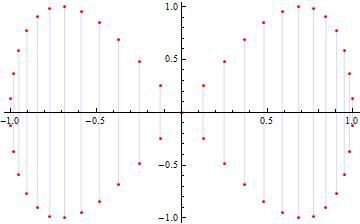
\includegraphics[width=.45\textwidth]{siivet.jpeg}
\end{center}
\label{kuvatus1}
\caption{Geronon lemniskaatta välillä $[-1,1]$.}
\end{figure}

\section{Tekstiä}

\lipsum[1-10]


%Kirjallisuusluettelon määrittelyssä {99} on levein kirjallisuusviitteen numero. Oikaise tarvittaessa.
 
\begin{thebibliography}{99}

\bibitem{NewtLeib} Newton ja Leibniz

\bibitem{Riemann} Riemann

\end{thebibliography}
